%\documentclass[convert={convertexe={magick.exe},size=1280}]{standalone}
\documentclass[border=3pt,tikz]{standalone}
\let\oldvec\vec
\usepackage{amsmath} % for \text
\usepackage{tikz}
\usepackage{comment}
\tikzset{>=latex} % for LaTeX arrow head
\usepackage{xcolor}
\colorlet{myblue}{black!40!blue}
\colorlet{myred}{black!40!red}

\providecommand{\sin}{} \renewcommand{\sin}{\hspace{2pt}\mathrm{sen}}
 
\begin{document}
% Adaptado de: https://wiki.physik.uzh.ch/cms/latex:tikz:electromagnetic_wave
% Electromagnetic wave - colored
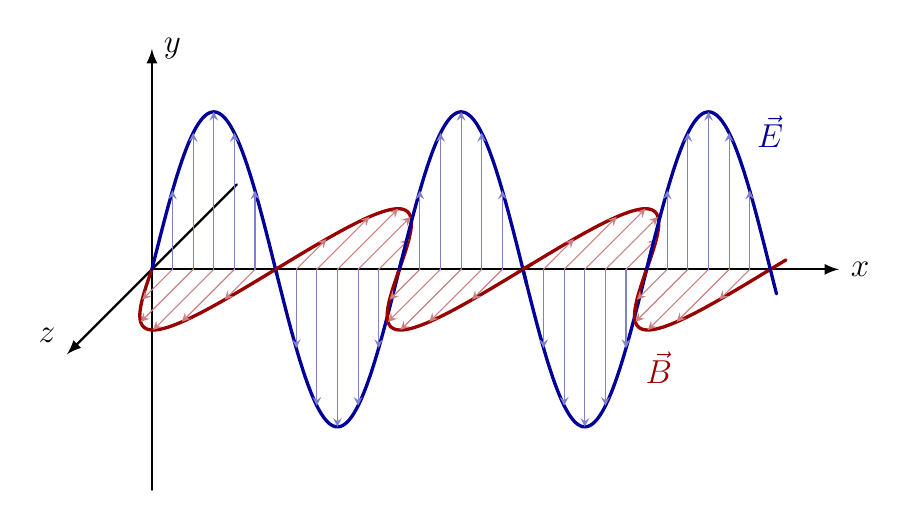
\begin{tikzpicture}[%x=(-15:1.2), y=(90:1.0), z=(-150:1.0), % rotações/distorções nos eixos, na forma polar
                    line cap=round, line join=round,
                    axis/.style={black, thick,->},
                    vector/.style={>=stealth,->}]
  \large
  \def\A{2} % Amplitude
  \def\nNodes{5} % Número de semi-ciclos
  \def\nVectorsPerNode{5} % Quantidade de vetores por semi-ciclo
  \def\N{\nNodes*40} % Quantidade de pontos a serem calculados para cada semi-ciclo
  \def\xmax{\nNodes*pi/2*1.01} % Valor máximo do eixo x
  \pgfmathsetmacro\nVectors{(\nVectorsPerNode+1)*\nNodes}

% Comando para desenhar um semiciclo da onda de campo elétrico
  \def\drawENode{ % draw E node and vectors with some offset
  % Desenha o semiciclo da senoide
    \draw[myblue, very thick, variable=\t, domain=\iOffset*pi/2:(\iOffset+1)*pi/2*1.01, samples=\N]
      plot (\t,{\A*sin(\t*360/pi)},0);
  % Desenha os vetores dentro da senoide
    \foreach \k [evaluate={\t=\k*pi/2/(\nVectorsPerNode+1);
                           \angle=\k*90/(\nVectorsPerNode+1);}]
                in {1,...,\nVectorsPerNode}{
      \draw[vector,myblue!50]  (\iOffset*pi/2+\t,0,0) -- ++(0,{\A*sin(2*\angle+\iOffset*180)},0);
    }
  }

% Comando para desenhar um semiciclo da onda de campo magnético
  \def\drawBNode{ % draw B node and vectors with some offset
  % Desenha o semiciclo da senoide
    \draw[myred, very thick ,variable=\t, domain=\iOffset*pi/2:(\iOffset+1)*pi/2*1.01, samples=\N]
      plot (\t,0,{\A*sin(\t*360/pi)});
  % Desenha os vetores dentro da senoide
    \foreach \k [evaluate={\t=\k*pi/2/(\nVectorsPerNode+1);
                           \angle=\k*90/(\nVectorsPerNode+1);}]
                in {1,...,\nVectorsPerNode}{
      \draw[vector,myred!50]  (\iOffset*pi/2+\t,0,0) -- ++(0,0,{\A*sin(2*\angle+\iOffset*180)});
    }
  }
 
% Desenha os eixos principais
  \draw[axis] (0,0,0) -- ++(\xmax*1.1,0,0) node[right] {$x$};
  \draw[axis] (0,-\A*1.4,0) -- (0,\A*1.4,0) node[right] {$y$};
  \draw[axis] (0,0,-\A*1.4) -- (0,0,\A*1.4) node[above left] {$z$};
 
% Desenha os semiciclos
  \foreach \iNode [evaluate={\iOffset=\iNode-1;}] in {1,...,\nNodes}{
    \ifodd\iNode \drawBNode \drawENode % E overlaps B
    \else        \drawENode \drawBNode % B overlaps E
    \fi
  }
  
% nome de cada onda
  \node[above right] at ({1.6*(\nNodes-2)*pi/2} , 0.7*\A , 0){\color{myblue}$\vec{E}$};
   \node[above right] at ({1.3*(\nNodes-2)*pi/2} , -0.8*\A , 0){\color{myred}$\vec{B}$};
\end{tikzpicture}

\end{document}